\documentclass[10pt, a4paper, italian]{article}
\usepackage[T1]{fontenc}
\usepackage[utf8]{inputenc}
\usepackage{amsmath, amssymb, amsthm, thmtools, amsfonts, mathtools}
\usepackage{nicefrac}
\usepackage{calc}
\usepackage[pdftex, hyperindex, plainpages=false]{hyperref}
\usepackage[nameinlink]{cleveref} %load before classicthesis (clash)
%\usepackage[nochapters,pdfspacing]{classicthesis}
\usepackage{siunitx}
\usepackage[siunitx]{circuitikz}

\usepackage[a4paper]{geometry}
\usepackage{float}
\usepackage{mdframed}
\usepackage{titling}
\usepackage{booktabs}
\usepackage{graphicx}
\usepackage{caption, subcaption}
\usepackage{xcolor}
\usepackage[italian]{babel}
\usepackage{pgfplots}
\usepackage{listings}
%\usepackage{lmodern}
\usepackage{url}
\usepackage{enumitem}
\usepackage{tikz} %loads after classicthesis (xcolor incompat)

% lets graphicx know path where figures to be included are found
\graphicspath{{../figs/}}
\makeatletter
\def\input@path{{../figs/}}
%or: \def\input@path{{/path/to/folder/}{/path/to/other/folder/}}
\makeatother

% tikz pgf plots setup
\usepgfplotslibrary{external}
\pgfplotsset{compat=1.15}
%\tikzexternalize

% spaces and significant digits/figures for measurements
\sisetup{free-standing-units, space-before-unit, number-unit-product = \;,
scientific-notation = false, round-mode = figures, round-precision = 1,}

% turns all (hyperlinked) references black [default is blue]
\hypersetup{
	linktoc=all,
	colorlinks=true,
	linkcolor=black
}

% code listings config
%\lstset{
%language=Python,
%basicstyle=\ttfamily,
%columns=fullflexible,
%keepspaces=true,
%}

% mdframed (for boxed text) configuration
\mdfsetup{linewidth=0.6pt}

% Default fixed font does not support bold face
\DeclareFixedFont{\ttb}{T1}{txtt}{bx}{n}{12} % for bold
\DeclareFixedFont{\ttm}{T1}{txtt}{m}{n}{12}  % for normal

% Custom colors
\usepackage{color}
\definecolor{deepblue}{rgb}{0,0,0.5}
\definecolor{deepred}{rgb}{0.6,0,0}
\definecolor{deepgreen}{rgb}{0,0.5,0}

% Commands 
\newcommand{\executeiffilenewer}[3]{%
	\ifnum\pdfstrcmp{\pdffilemoddate{#1}}%
		{\pdffilemoddate{#2}}>0%
	{\immediate\write18{#3}}\fi%
}
% input .svg --> .pdf_tex graphs
%\newcommand{\includesvg}[1]{%
%	\executeiffilenewer{#1.svg}{#1.pdf}%
%	{inkscape -z -D --file=#1.svg %
%	--export-pdf=#1.pdf --export-latex}%
%	\input{#1.pdf_tex}%
%}
% Thanks UniPi's Department of Physics E. Fermi
\newcommand{\thanksdf}{(\thanks{Dipartimento di Fisica E.~Fermi,%
Universit\`a di Pisa - Pisa, Italy.}\;)}

% hyperlink to email address
\newcommand{\mail}[1]{\href{mailto:#1}{\textsf{#1}}}

% \vec for bold vectors, instead of overarrows (now "\arrvec")
\let\arrvec=\vec
\renewcommand{\vec}[1]{\boldsymbol #1}
% replaces straight phi with slanted phi
\renewcommand{\phi}{\varphi}
% replaces straight eps with curved epsilon
\newcommand{\eps}{\varepsilon}
% abbreviation for (sub_/super^)scripts of \lim, \sum,... in inline math
\newcommand{\ds}{\displaystyle}

% blackboard/number set letters
\newcommand{\CC}{\mathbb C}
\newcommand{\HH}{\mathbb H}
\newcommand{\KK}{\mathbb K}
\newcommand{\NN}{\mathbb N}
\newcommand{\PP}{\mathbb P}
\newcommand{\QQ}{\mathbb Q}
\newcommand{\RR}{\mathbb R}
\newcommand{\ZZ}{\mathbb Z}

\newcommand{\Abs}[1]{{\left\Vert #1\right\Vert}}
\newcommand{\enclose}[1]{{\left( #1 \right)}}
\newcommand{\Enclose}[1]{{\left[ #1 \right]}}
\newcommand{\floor}[1]{\left\lfloor #1 \right\rfloor}
\newcommand{\ceil}[1]{\left\lceil #1 \right\rceil}
\newcommand{\To}{\rightrightarrows}

% Math operators
\DeclareMathOperator{\divergence}{div}
\renewcommand{\div}{\divergence}
\DeclareMathOperator{\Imaginarypart}{Im}
\renewcommand{\Im}{\Imaginarypart}
\DeclareMathOperator{\Realpart}{Re}
\renewcommand{\Re}{\Realpart}
%\DeclareMathOperator{\arg}{arg}
\DeclareMathOperator{\tg}{tg}
\DeclareMathOperator{\arctg}{arctg}
\DeclareMathOperator{\settsinh}{settsinh}
\DeclareMathOperator{\settcosh}{settcosh}
\DeclareMathOperator{\tr}{tr}
\DeclareMathOperator{\im}{im}
\DeclareMathOperator{\sgn}{sgn}
\DeclareMathOperator{\diag}{diag}

\DeclarePairedDelimiter{\norm}{\lVert}{\rVert}
\DeclarePairedDelimiter{\scalar}{\langle}{\rangle}

% Logarithm with arbitrary base.
% -> log_10
\newcommand{\llog}[1][10]{\log_{#1}}

% Absolute value.
% -> |x|
\newcommand{\abs}[1]{\left| #1 \right|}

% Powers.
% -> x^a
\newcommand{\power}[2][2]{\left( #2 \right)^{#1}}

% Square.
% -> x^2
\newcommand{\sq}[1]{\power[2]{#1}}

% Expansion of the binomial coefficient.
% -> n1!/(n2!(n1 - n2)!)
\newcommand{\binomexpr}[2]{\frac{#1!}{#2!(#1 - #2)!}}

% Expression evaluation at a given point with square brackets.
% -> [x]_{a}
\newcommand{\at}[2]{\left[ #1\right]_{\makebox[-1pt][l]{${\scriptstyle#2}$}}}

% Expression evaluation in an interval.
% -> [x] _{a}^{b}
\newcommand{\eval}[3]{\left.#1%
  \right|_{\makebox[-1pt][l]{${\scriptstyle#2}$}}^{\makebox[-1pt][l]{${\scriptstyle#3}$}}}

% Upright d in math mode (for differentials).
% -> d
\newcommand{\ud}{\mathrm{d}}

% Differential.
% -> dx
\newcommand{\diff}[1][x]{\,\ud{#1}}

% Base command for defining derivatives.
% -> df/dx or d^kf/dx^k
\newcommand{\basederivative}[4][]{%
  \displaystyle%
  \ifx\\#1\\\frac{#4#2}{#4#3}%
  \else%
  \frac{#4^#1#2}{#4#3^#1}%
  \fi%
}

% Total derivative.
% -> df/dx(x) or d^kf/dx^k(x)
\newcommand{\td}[4][]{%
  \basederivative[#1]{#2}{#3}{\ud}%
  \ifx\\#4\\%
  \else%
  \mkern-4mu\left(#4\right)%
  \fi%
}

% Partial derivative.
% -> df/dx(x) or d^kf/dx^k(x)
\newcommand{\pd}[4][]{%
  \basederivative[#1]{#2}{#3}{\partial}%
  \ifx\\#4\\%
  \else%
  \mkern-4mu\left(#4\right)%
  \fi%
}

\newcommand{\intinf}{\int_{-\infty}^{\infty}\!\!\!}

\newcommand{\cinterval}[2]{\left[\, #1,~#2 \,\right]}

\newcommand{\linterval}[2]{\left[\, #1,~#2 \,\right)}

\newcommand{\rinterval}[2]{\left(\, #1,~#2 \,\right]}

\newcommand{\ointerval}[2]{\left(\, #1,~#2 \,\right)}

\newcommand{\prob}[1]{\displaystyle P\left(#1\right)}

\newcommand{\pvalue}{\emph{$p$-value}}

\newcommand{\cond}{\,|\,}

\newcommand{\expect}[1]{\displaystyle E\left[#1\right]}

\newcommand{\mom}[2][]{\displaystyle {\cal M}_{#2}\ifx\\#1\\\else(#1)\fi}

\newcommand{\momalg}[1]{\displaystyle \lambda_{#1}}

\newcommand{\momcen}[1]{\displaystyle \mu_{#1}}

\newcommand{\skewness}{\displaystyle \gamma_1}

\newcommand{\kurtosis}{\displaystyle \gamma_2}

\newcommand{\charf}[1][x]{\phi_{#1}}

\newcommand{\momgenf}[1][x]{M_{#1}}

\newcommand{\fwhm}{{\scriptstyle \textsc{FWHM}}}

\newcommand{\hwhm}{{\scriptstyle \textsc{HWHM}}}

\newcommand{\median}{\mu_{\nicefrac{1}{2}}}

\newcommand{\var}[1]{\ensuremath{\text{Var}\left(#1\right)}}

\newcommand{\cov}[2]{\ensuremath{\text{Cov}\left(#1, #2\right)}}

\newcommand{\corr}[2]{\ensuremath{\text{Corr}\left(#1, #2\right)}}

\newcommand{\like}{\mathcal L}

\newcommand{\likelihood}[2][]{\like\ifx\\#2\\\else(#2\ifx\\#1\\\else;#1\fi)\fi}

\newcommand{\chisq}{\ensuremath{\chi^2}}

\newcommand{\chisquare}[2][]{\chisq\ifx\\#2\\\else(#2\ifx\\#1\\\else;#1\fi)\fi}

\newcommand{\loglikelihood}[2][]{\log\likelihood[#1]{#2}}

\newcommand{\pdf}[3][]{#2(#3\ifx\\#1\\\else;#1\fi)}

\newcommand{\binomialpdf}[2][]{\pdf[#1]{\mathcal B}{#2}}

\newcommand{\multinomialpdf}[2][]{\pdf[#1]{\mathcal M}{#2}}

\newcommand{\poissonpdf}[2][]{\pdf[#1]{\mathcal P}{#2}}

\newcommand{\uniformpdf}[2][]{\pdf[#1]{u}{#2}}

\newcommand{\exponentialpdf}[2][]{\pdf[#1]{\varepsilon}{#2}}

\newcommand{\gausspdf}[2][]{\pdf[#1]{N}{#2}}

\newcommand{\chisquarepdf}[2][]{\pdf[#1]{\wp}{#2}}

\newcommand{\cauchypdf}[2][]{\pdf[#1]{c}{#2}}

\newcommand{\erf}[1]{\ensuremath{\text{erf}\left(#1\right)}}

\newcommand{\dccases}[4][]{#2 \ifx\\#2\\\else=\fi %
  \begin{cases}
    \displaystyle #3 & \text{per variabili discrete}\\
    \displaystyle #4 & \text{per variabili continue}#1
  \end{cases}
}
% sub/super-scriptable for all symbol as math operator 
\newcommand\Scaleforall[1]{\vcenter{\hbox{\scalefont{#1}$\forall$}}}

\DeclareMathOperator*\forevery{%
  \vphantom\sum
  \mathchoice{\Scaleforall{2}}{\Scaleforall{1.4}}{\Scaleforall{1}}{\Scaleforall{0.75}}}
\geometry{left=2cm, right=2cm, top=2cm, bottom=2cm}

% indexes subsections with letters, sections with numbers (1.a, 1.b, ...)
\renewcommand{\thesubsection}{\thesection.\alph{subsection}}

% lets graphicx know path where figures to be included are found
\graphicspath{{../figs/}}

\author{Gruppo 1.AC \\ Matteo Rossi, Bernardo Tomelleri}
\title{EsD0: Funzionalità di Waveforms per segnali digitali}
\begin{document}
\date{\today}
\maketitle

\setcounter{section}{0}

\section{Misura componenti dei circuiti}
\begin{table}[htbp]
\centering
\begin{tabular}{cccccc}
\toprule
Resistenze $[\si{\ohm}]$ & $R$ & $\sigma R$ & Capacità $[\si{\F}]$ & $C$ &
$\sigma C$ \\
\midrule
\midrule
$R_1$	  & 100 	& 1 	 & $C\ped{in}$ & 95	n	 & 4 n \\
$R_S$	  & 219	& 3 	 & $C\ped{out}$ & 9.6 n	 & 0.4 n \\
$R_D$	  & 997		& 8	 	 & $C_S$ 		& 95  µ  & 5 µ \\
$R_G$	  & 1.02 M	& 0.1 M	 & & & \\
$R_s$	  & 99.6 k	& 0.8 k	 & & & \\
\bottomrule     
\end{tabular}
\caption{Valori di resistenza e capacità misurate per i componenti dei
circuiti studiati. \label{tab: rcmes_M}}
\end{table}

\begin{table}[htbp]
\centering
\begin{tabular}{cccccc}
\toprule
Resistenze $[\si{\ohm}]$ & $R$ & $\sigma R$ & Capacità $[\si{\F}]$ & $C$ &
$\sigma C$ \\
\midrule
\midrule
$R_1$	  & 100.2 	& 0.9 	 & $C\ped{in}$ & 99	n	 & 4 n \\
$R_S$	  & 217	& 3 	 & $C\ped{out}$ & 10.4 n	 & 0.4 n \\
$R_D$	  & 993		& 8	 	 & $C_S$ 		& 96  µ  & 4 µ \\
$R_G$	  & 994 k	& 8	 & & & \\
$R_s$	  & 996 k	& 8	 & & & \\
\bottomrule     
\end{tabular}
\caption{Valori di resistenza e capacità misurate per i componenti dei
circuiti studiati. \label{tab: rcmes_B}}
\end{table}

Riportiamo per completezza anche i valori delle tensioni di alimentazione
continue per gli op-amp misurate con il multimetro
\begin{align*}
V_{DD} &= 4.99 \pm 0.03 \si{\V} \\
V_{SS} &= -4.99 \pm 0.03 \si{\V}
\end{align*}

\subsection*{Nota sul metodo di fit}
Per determinare i parametri ottimali e le rispettive covarianze si \`e
implementato in \verb+Python+ un algoritmo di fit basato sui minimi quadrati
mediante la funzione \emph{curve\_fit} della libreria \texttt{SciPy}.

%=======================
\section{Studio del funzionamento}
Come primo passo abbiamo verificato il corretto funzionamento del JFET a canale
N 2N3819 studiandone le caratteristiche dalla configurazione circuitale
riportata in \ref{schm: tracer}
\begin{figure}[htbp]
    \centering
	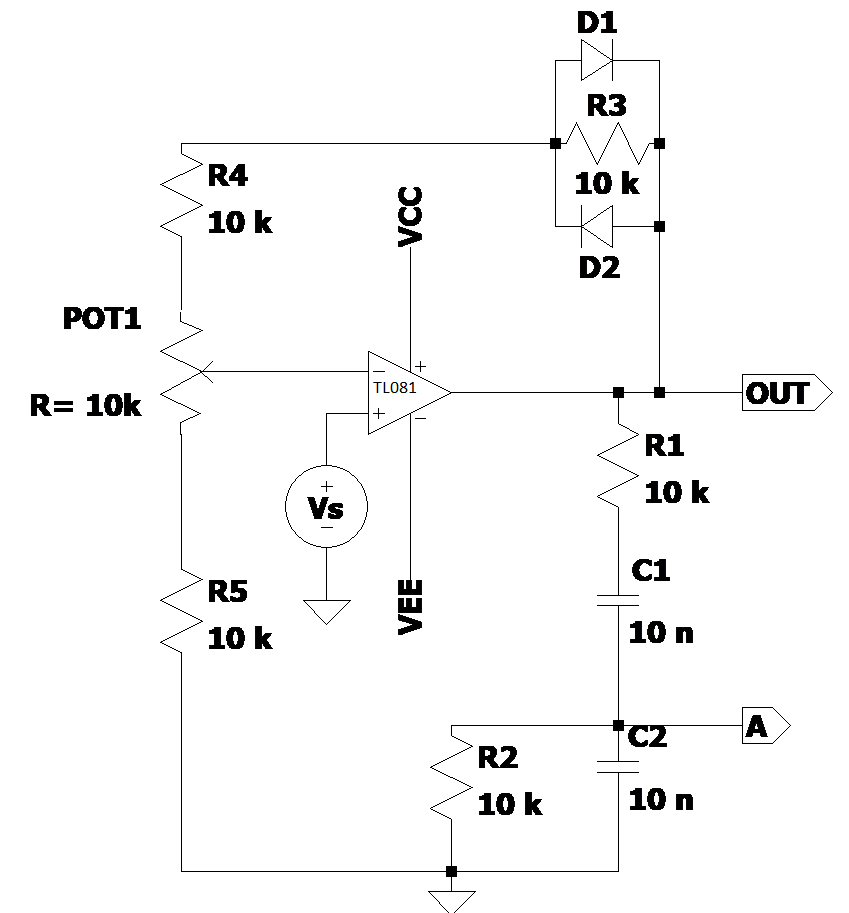
\includegraphics[scale=0.5]{Draft1}
    \caption{Schema circuitale per la verifica di funzionamento del JFET
    \label{schm: tracer}}
\end{figure}

Dal nostro modello sulla struttura del JFET sappiamo che all'aumentare di
$V_{GS}$ (in negativo verso $V_{SS} = \SI{-5}{\V})$ le zone della giunzione
vengono svuotate dai portatori di carica, fino a che non si raggiunge una
tensione di pinch-off $V_p$. Per valori di tensione $V_{GS} < V_P$ il canale
risulta completamente svuotato e la corrente di drain $I_{DS}$ tende a 0,
condizione che indichiamo con il nome regime di interdizione.
Al contrario, quando $V_{GS} = \SI{0}{\V}$ il canale risulta ``aperto'', quindi
ci aspettiamo di trovare in questa situazione la massima intensità di corrente
che può scorrere attraverso il transistor.

\subsection{Curve tracer}
Abbiamo applicato al gate una tensione di polarizzazione continua
$V_{SS}$ di -5 V in modo da polarizzare inversamente la giunzione
$\text{np}^+$ (gate-canale).
Dunque si invia in WG1 una rampa a scalini equispaziati di 250 mV partendo
da -5 V fino a 0 V, mentre in WG2 per ogni gradino step di WG1 si genera una
rampa che parte dal valore corrente di WG1 e arriva fino a 5 V.
Di seguito quello che otteniamo dall'oscilloscopio.
\begin{figure}[htbp]
    \centering
	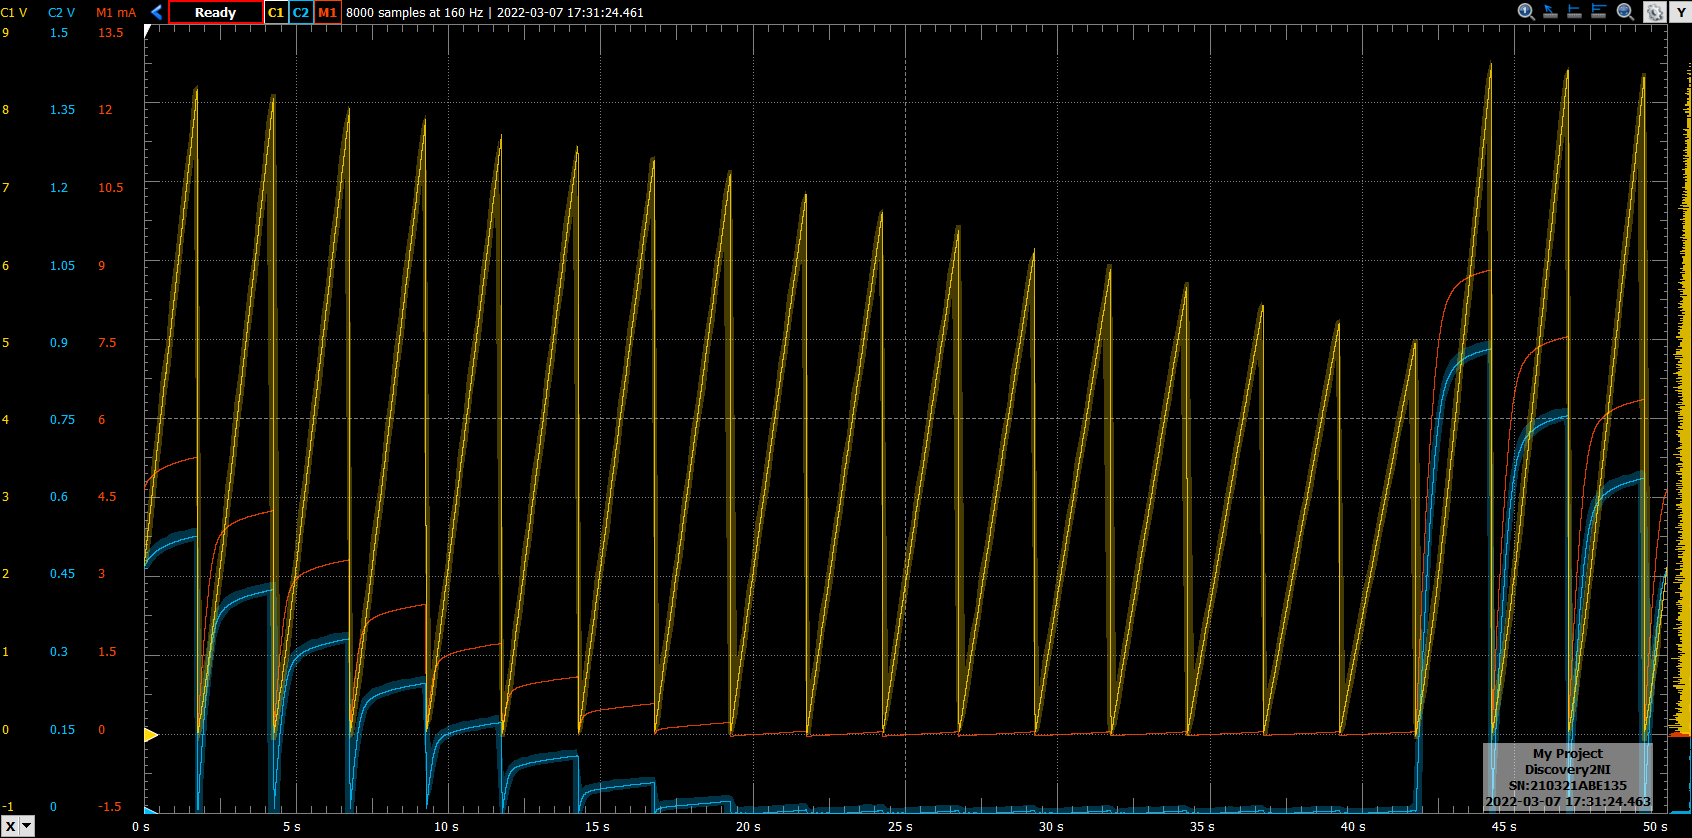
\includegraphics[width=\textwidth]{timey}
    \caption{Acquisizione all'oscilloscopio di $V_{DS}$ (CH1), $V_{R_1}$ (CH2)
    e $I_{DS} = V_{R_1}/R_1$ in funzione del tempo \label{fig: ramp}}
\end{figure}

Notiamo esplicitamente come $V_{DS}$ risulta sempre positivo, mentre $V_{GS}$
è sempre negativo, in accordo con le condizioni $V_{DS} > 0$ e $V_{GS} < 0$
da verificare.

\subsection{Curve caratteristiche ottenute}
Riportiamo inoltre i grafici ottenuti di $I_{DS}$ vs $V_{DS}$, ovvero le
curve caratteristiche di collettore del JFET dall'alto verso il basso in
ordine decrescente di $V_{GS} \in [0, -5]\; \si{V}$.
\begin{figure}[htbp]
    \centering
	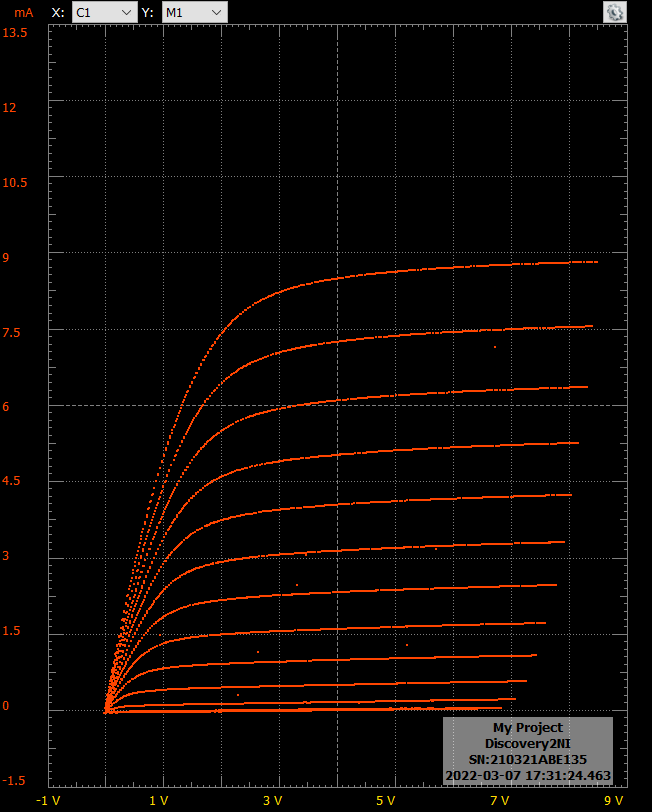
\includegraphics[scale=0.6]{xy}
    \caption{Curve caratteristiche di $I_{DS}$ in funzione di $V_{DS}$ al
    variare di $V_{GS}$ tra $-5$ e $\SI{0}{\V}$ per il primo JFET.
    \label{fig: IDS-VDS1}}
\end{figure}
\begin{figure}[htbp]
    \centering
	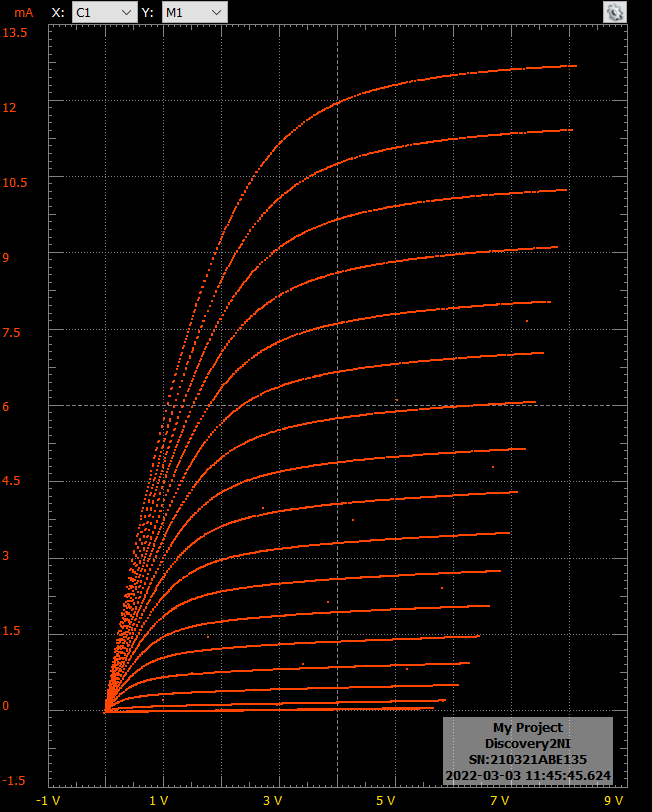
\includegraphics[scale=0.6]{vgs}
    \caption{Curve caratteristiche di $I_{DS}$ in funzione di $V_{DS}$
    al variare di $V_{GS}$ tra $-5$ e $\SI{0}{\V}$ per il secondo JFET.
    \label{fig: IDS-VDS2}}
\end{figure}

\subsection{Confronto con datasheet}
A conferma di quanto detto prima, si registra la massima intensità di corrente
quando $V_{GS} = \SI{0}{\V}$, che come si può vedere dalla \cref{fig: ramp}
(in particolare nel grafico vedere l'andamento di CH2)
corrisponde al momento in cui la rampa di WG2 misurata da CH1 è alla sua
massima ampiezza (perchè in quel caso $V_S$ è pari a $V_G$ ovvero $V_{SS}$).

Inoltre si può vedere che oltre un certo punto l'andamento di CH2 risulta
approssimativamente costante: questo si ottiene quando viene superata la
tensione di pinch-off, che abbiamo misurato tramite cursori:
\begin{align*}
V_p &= -3.0 \pm 0.2 \; \si{\V} \\
V_p &= -4.0 \pm 0.2 \; \si{\V}
\end{align*}
dove abbiamo preso come incertezza associata il passo dei nostri scalini di
tensione (0.25 V).

Infine, sempre utilizzando i cursori, abbiamo misurato l'intensità di corrente
della traccia per cui vale $V_{GS} = 0$ (nel grafico \ref{fig: IDS-VDS1} è
la curva più alta; da cui si trova:
\begin{align*}
I_{DSS} &= 8.62 \pm 0.07 \; \si{m\A} \\
I_{DSS} &= 12.6 \pm 0.2 \; \si{m\A}
\end{align*}
Confrontando i risultati ottenuti dalla nostra analisi con quanto riportato
nel datasheet troviamo che entrambi i valori sono compatibili con gli
intervalli dichiarati dai costruttori (dal momento che noi prendiamo in
considerazione valori di $V_{DS}$ minori di quelli presi di riferimento nel
datasheet).

%=======================
\section{Amplificatore di tensione e punto di lavoro}
A questo punto abbiamo costruito il circuito per l'amplificatore di tensione:
\begin{figure}[htbp]
    \centering
	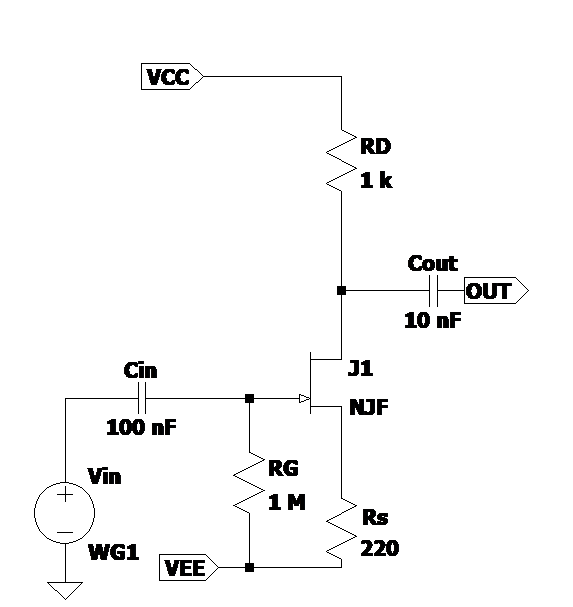
\includegraphics[scale=0.7]{Draft2}
    \caption{Schema circuitale per l'amplificazione di segnale tramite JFET}
\end{figure}
Quindi si è collegato $V_{DD}$ a 5V e $V_{SS}$ a -5V tenendo scollegato
$v\ped{in}$ per individuare il punto di lavoro del JFET.

\subsection{Corrente di quiescenza}
Misurando la caduta di potenziale ai capi della resistenza $R_D$ abbiamo
ricavato la corrente di quiescenza tramite la legge di ohm, da cui si ha
\begin{align*}
I_{DS}^Q &= 4.06 \pm 0.05 \; \si{m\A} \\
I_{DS}^Q &= 6.42 \pm 0.08 \; \si{m\A}
\end{align*}
che risultano essere circa la metà delle rispettive $I_{DSS}$, come voluto
per avere regime di linearità più ampio possibile al variare di $v\ped{in}$.

Si è quindi proseguito con la misura di $V_{GS}$ e di $V_{DS}$ per poter
confrontare il valore di $I_{DS}$ appena trovato con il suo valore atteso
quando il JFET è in regime di saturazione:
\begin{equation}\label{eq: IDS}
I_{DS} = \frac{I_{DSS}}{V_p ^2}(V_{GS} - V_p)^2
\end{equation}

\subsection{Tensioni ai terminali del JFET}
Non potendo misurare direttamente la differenza di potenziale tra gate e
source a causa dell'elevata impedenza in ingresso del JFET (per cui
l'inserimento in parallelo di uno strumento di misura perturberebbe in
maniera non trascurabile il circuito) per misurare $V_{GS}$ si è calcolata la
differenza tra le misure di $V_G$ e $V_S$:
\begin{align*}
V_{GS} &= -886 \pm 7 \; \si{m\V} \\
V_{DS} &= 2.35 \pm 0.01 \; \si{\V}
\end{align*}

mentre per il secondo JFET risulta:
\begin{align*}
V_{GS} &= -994 \pm 8 \; \si{m\V} \\
V_{DS} &= 2.10 \pm 0.02 \; \si{\V}
\end{align*}
Dal momento che è soddisfatta la condizione $V_{DS} > V_{GS} - V_p$ notiamo che
siamo in zona di saturazione nel caso del primo JFET, mentre il secondo sembra
ancora trovarsi in zona ohmica. Quindi possiamo confrontare il valore di
$I_{DS}^Q$ previsto dall'\cref{eq: IDS} solo per il primo, da cui risulta 
\[
I_{DS}(V_{GS},V_p,I_{DSS}) = 4.3 \pm 0.4 \; \si{m\A}
\]
che risulta compatibile con quanto misurato.

Dato che il secondo JFET non sembra essere entrato in saturazione impieghiamo
invece la seguente formula per stimare $I_{DS}$ nella regione ohmica:
\begin{equation}
I_{DS} = \frac{I_{DSS}}{V_P^2}[2(V_{GS}-V_P) - V_{DS}]V_{DS} =
6.47 \pm 0.06 \; \si{m\A}
\end{equation}
che risulta pienamente compatibile con la misura di $I_{DS}$ sul secondo JFET.

\subsection{Stima della transconduttanza $g_m$}
Stimiamo infine la transconduttanza nel punto di lavoro grazie alla formula
\begin{equation}\label{eq: gm}
g_m = \frac{2 I_{DSS}}{|V_p|}\sqrt{\frac{I_{d}}{I_{DSS}}}
\end{equation}
da cui otteniamo i nostri valori indirettamente misurati
\begin{align*}
g_m &= 3.9 \pm 0.3 \; \si{m\mho} \\
g_m &= 4.5 \pm 0.2 \; \si{m\mho}
\end{align*}

A questo punto abbiamo invece provato a misurare la stessa $g_m$ dal grafico,
dal rapporto tra la differenza nella corrente $I_{DS} $ e la differenza di
potenziale di $V_{GS}$ tra le 2 curve associate più vicine al punto di lavoro
(vista la "risoluzione" di 250 mV abbiamo preso come punti per effettuare la
misura $V_{GS}= -0.75 \; \si{\V}$ e $V_{GS}= -1 \; \si{\V}$)
(a parità di $V_{DS}$) da cui si trova:
\begin{align*}
g_m &= 3.92 \pm 0.05 \; \si{m\mho} \\
g_m &= 4.49 \pm 0.05 \; \si{m\mho}
\end{align*}

Successivamente siamo andati a ricercare nel datasheet il valore fornito dal
costruttore, in cui troviamo un grafico di $g_m$ in funzione della frequenza
a cui opera il JFET. In particolare notiamo che per frequenze minori di circa
500 MHz la transconduttanza deve essere compresa approssimativamente tra 4 e
$\SI{5}{m\mho}$, similmente anche la transammettenza deve essere compresa tra
3 e 6.5 $\si{m\mho}$.

I valori da noi misurati sono quindi compatibili sia con quelli riportati nel
datasheet che con quelli ricavati dall'\cref{eq: gm}.

%=======================
\section{Amplificazione di piccoli segnali a frequenza fissa}
A questo punto si è collegato WG1 all'ingresso dell'amplificatore e lo
abbiamo pilotato con un'onda sinusoidale di frequenza fissata a
$f = 1 \; \si{k\Hz}$. Al variare dell'ampiezza $v\ped{in}$ tra 100 mV e 2.8 V
a passi di 100 mV, dall'ampiezza (e la fase) della risposta in uscita
$v\ped{out}$ abbiamo misurato il guadagno $A_v = \frac{v\ped{out}}{v\ped{in}}$
\begin{table}[H]
\centering
\begin{tabular}{cccccc}
\toprule
$v\ped{in} [V]$ & $\sigma v\ped{in}[V]$ & $v\ped{out} [V]$ &
$\sigma v\ped{out} [V]$ & $|A_v|$ & $\sigma A_v$ \\
\midrule
\midrule
100 m & 1 m  & 206 m & 2 m   & 2.06 & 0.02 \\
200 m & 2 m  & 411 m & 4 m   & 2.05 & 0.02 \\
300 m & 3 m  & 616 m & 7 m  & 2.05 & 0.03 \\
400 m & 4 m  & 821 m & 7 m  & 2.05 & 0.02 \\
501 m & 4 m  & 1.03  & 8 m  & 2.05 & 0.02 \\
601 m & 7 m  & 1.22  & 18 m & 2.04 & 0.04 \\
701 m & 7 m  & 1.42  & 19 m & 2.03 & 0.03 \\
801 m & 7 m  & 1.62  & 20 m & 2.02 & 0.03 \\
901 m & 7 m  & 1.80  & 0.02 & 2.00 & 0.03 \\
1.00  & 8 m  & 1.99  & 0.02 & 1.99 & 0.03 \\
1.10  & 8 m  & 2.16  & 0.02 & 1.96 & 0.02 \\
1.20  & 8 m  & 2.31  & 0.02 & 1.93 & 0.02 \\
1.30  & 9 m  & 2.46  & 0.02 & 1.89 & 0.02 \\
1.40  & 9 m  & 2.59  & 0.03 & 1.86 & 0.02 \\
1.50  & 0.02 & 2.71  & 0.04 & 1.82 & 0.03 \\
1.60  & 0.02 & 2.84  & 0.04 & 1.78 & 0.03 \\
1.70  & 0.02 & 2.93  & 0.04 & 1.72 & 0.03 \\
1.80  & 0.02 & 3.05  & 0.04 & 1.69 & 0.03 \\
1.90  & 0.02 & 3.15  & 0.04 & 1.65 & 0.03 \\
2.00  & 0.02 & 3.25  & 0.04 & 1.62 & 0.03 \\
2.10  & 0.02 & 3.34  & 0.04 & 1.59 & 0.02 \\
2.20  & 0.02 & 3.48  & 0.04 & 1.56 & 0.02 \\
2.30  & 0.02 & 3.53  & 0.04 & 1.53 & 0.02 \\
2.40  & 0.02 & 3.59  & 0.04 & 1.49 & 0.02 \\
2.50  & 0.02 & 3.61  & 0.04 & 1.44 & 0.02 \\
2.60  & 0.03 & 3.63  & 0.04 & 1.39 & 0.02 \\
2.71  & 0.03 & 3.63  & 0.04 & 1.34 & 0.02 \\
2.81  & 0.04 & 3.64  & 0.04 & 1.29 & 0.02 \\
\bottomrule
\end{tabular}
\end{table}

Per l'amplificatore invertente con JFET in configurazione a emettitore comune
ci aspettiamo un valore di guadagno dato dalla formula
\begin{equation}\label{eq: Av}
A_v = -\frac{g_m R_D}{1 + g_m R_S} = -2.10 \pm 0.03
\end{equation}

Ci accorgiamo subito che questo non risulta compatibile in modulo con quanto
misurato (a piccole ampiezze di segnale), mentre dal segno negativo ci
aspettiamo che l'amplificatore sia di tipo invertente, come ben visibile dalle
acquisizioni di $v\ped{in}$ e $v\ped{out}$ all'oscilloscopio riportate sotto.

Infatti, se i due segnali sono in opposizione di fase il passaggio per 0 con
la stessa pendenza/slope devono distare un semi-periodo dall'altro; per cui ai
massimi del segnale in ingresso (la traccia gialla) corrispondono i minimi del
segnale in uscita (la traccia blu)

Da una misura con i cursori troviamo
\begin{align*}
\Delta t &= 50.2 \pm 1.0 \; \si{n\s} \\
\Delta \phi &= 2\pi f \Delta t = 3.14 \pm 0.06 \; \si{\radian}
\end{align*}
mentre con la funzione di misura automatica definita con uno script di Wavegen
risulta:
\[
\phi = 179.4 \pm 0.5 \; \si{\degree}
\]
che sono entrambi compatibili con il valore atteso di $\Delta \phi\ped{exp}
= \pi \; \si{\radian}$ per la natura invertente dell'amplificatore.
\begin{figure}[htbp]
    \centering
	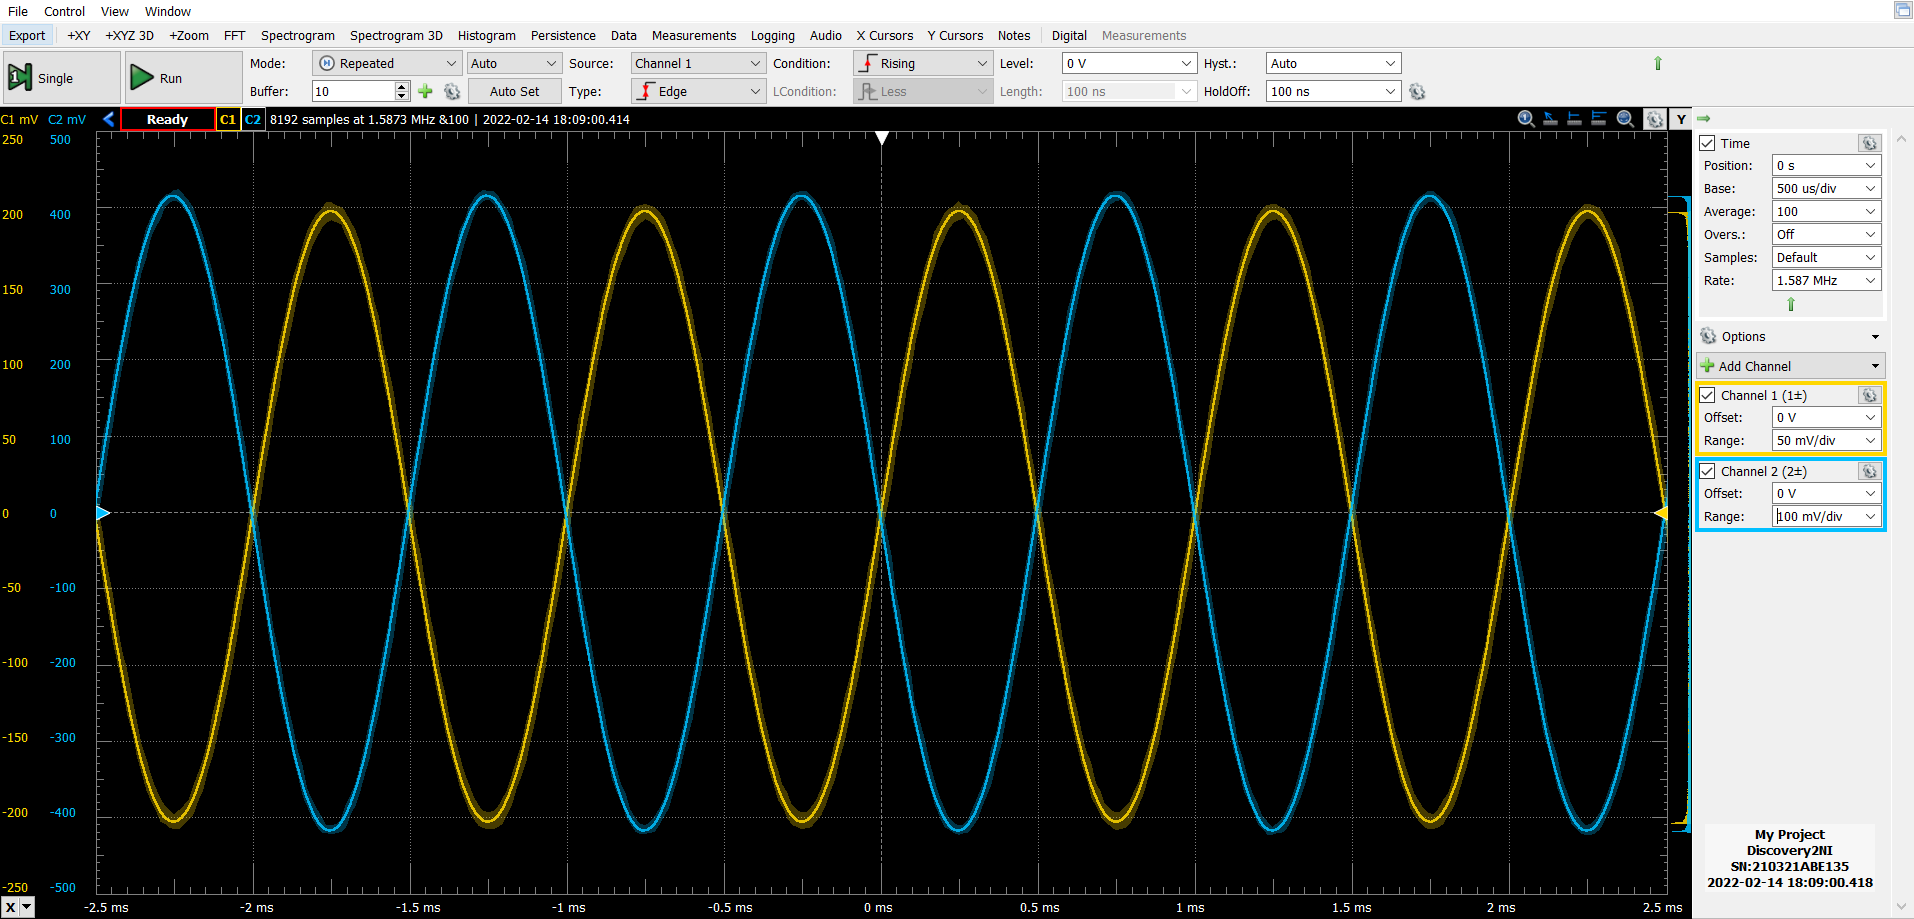
\includegraphics[width=\textwidth]{amp.200}
    \caption{Acquisizione all'oscilloscopio di $v\ped{in} (t)$ (CH1) e
    $v\ped{out} (t)$ (CH2) in funzione del tempo con ampiezza
    $v\ped{in} = 200 \; \si{m\V}$}
\end{figure}
\begin{figure}[htbp]
    \centering
	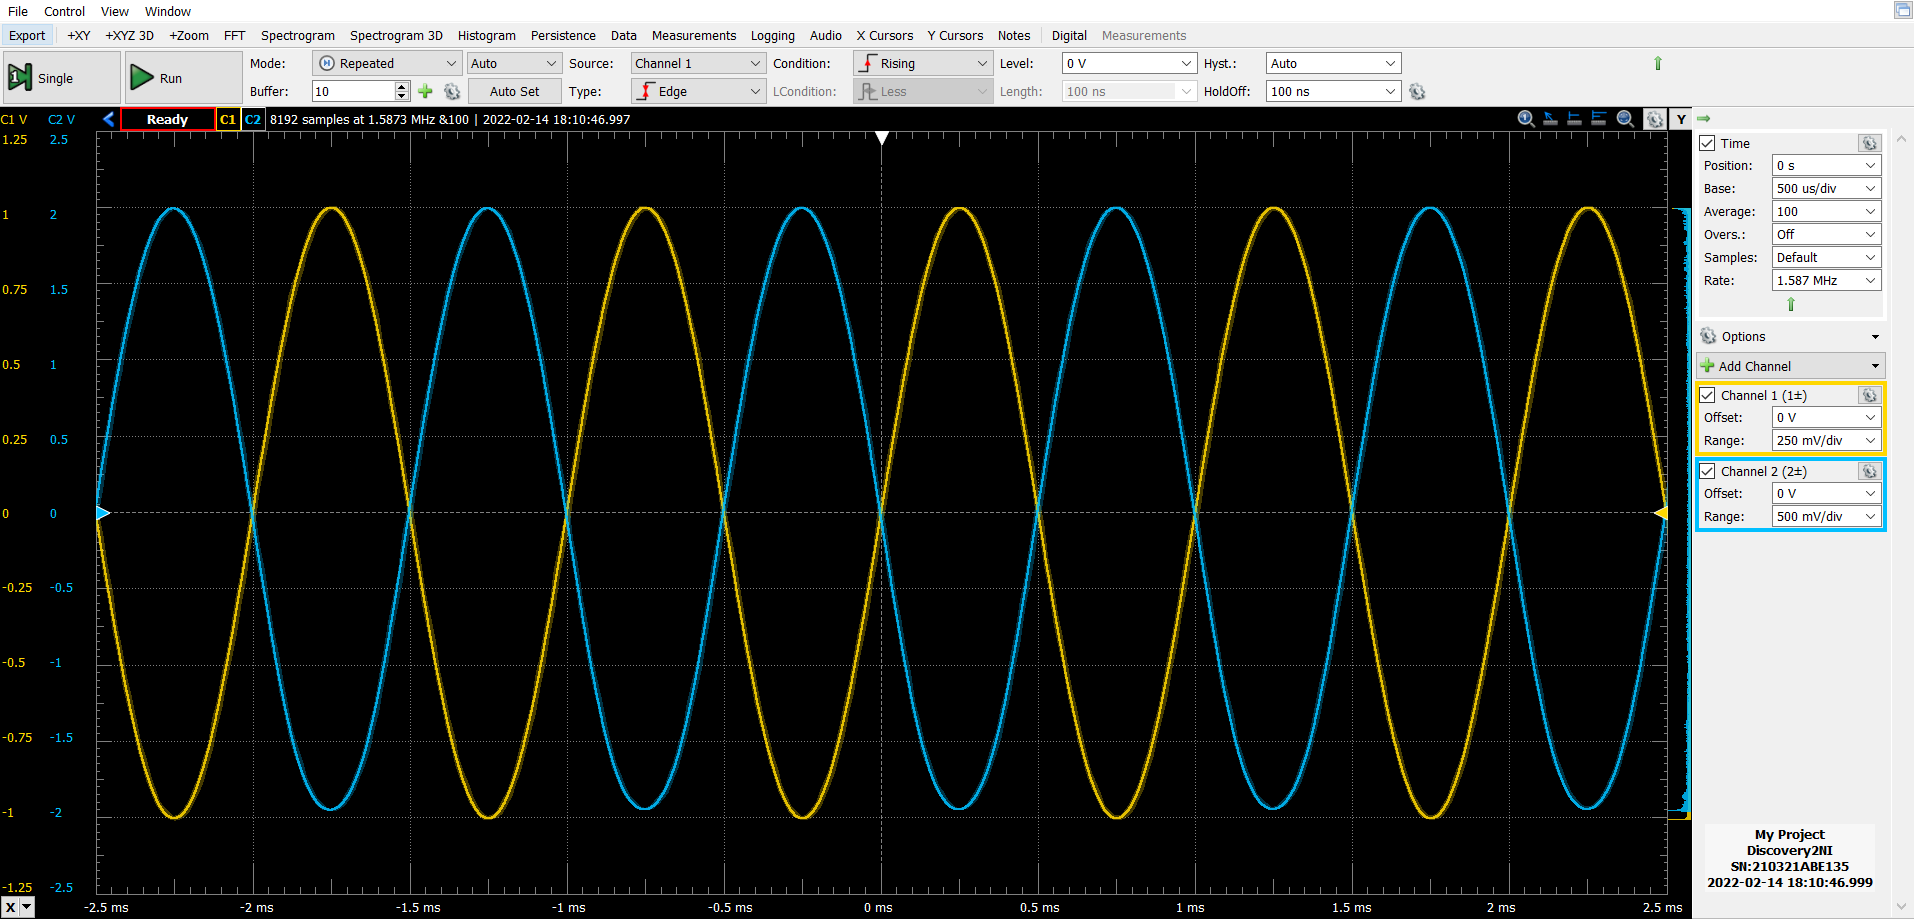
\includegraphics[width=\textwidth]{amp.1000}
    \caption{Acquisizione all'oscilloscopio di $v\ped{in} (t)$ (CH1) e
    $v\ped{out} (t)$ (CH2) in funzione del tempo con ampiezza
    $v\ped{in} = 1 \; \si{\V}$. In cui si nota una distorsione nel segnale
    in uscita, in particolare la parte inferiore dell'onda risulta
    ``schiacciata'' verso lo 0.}
\end{figure}
\begin{figure}[htbp]
    \centering
	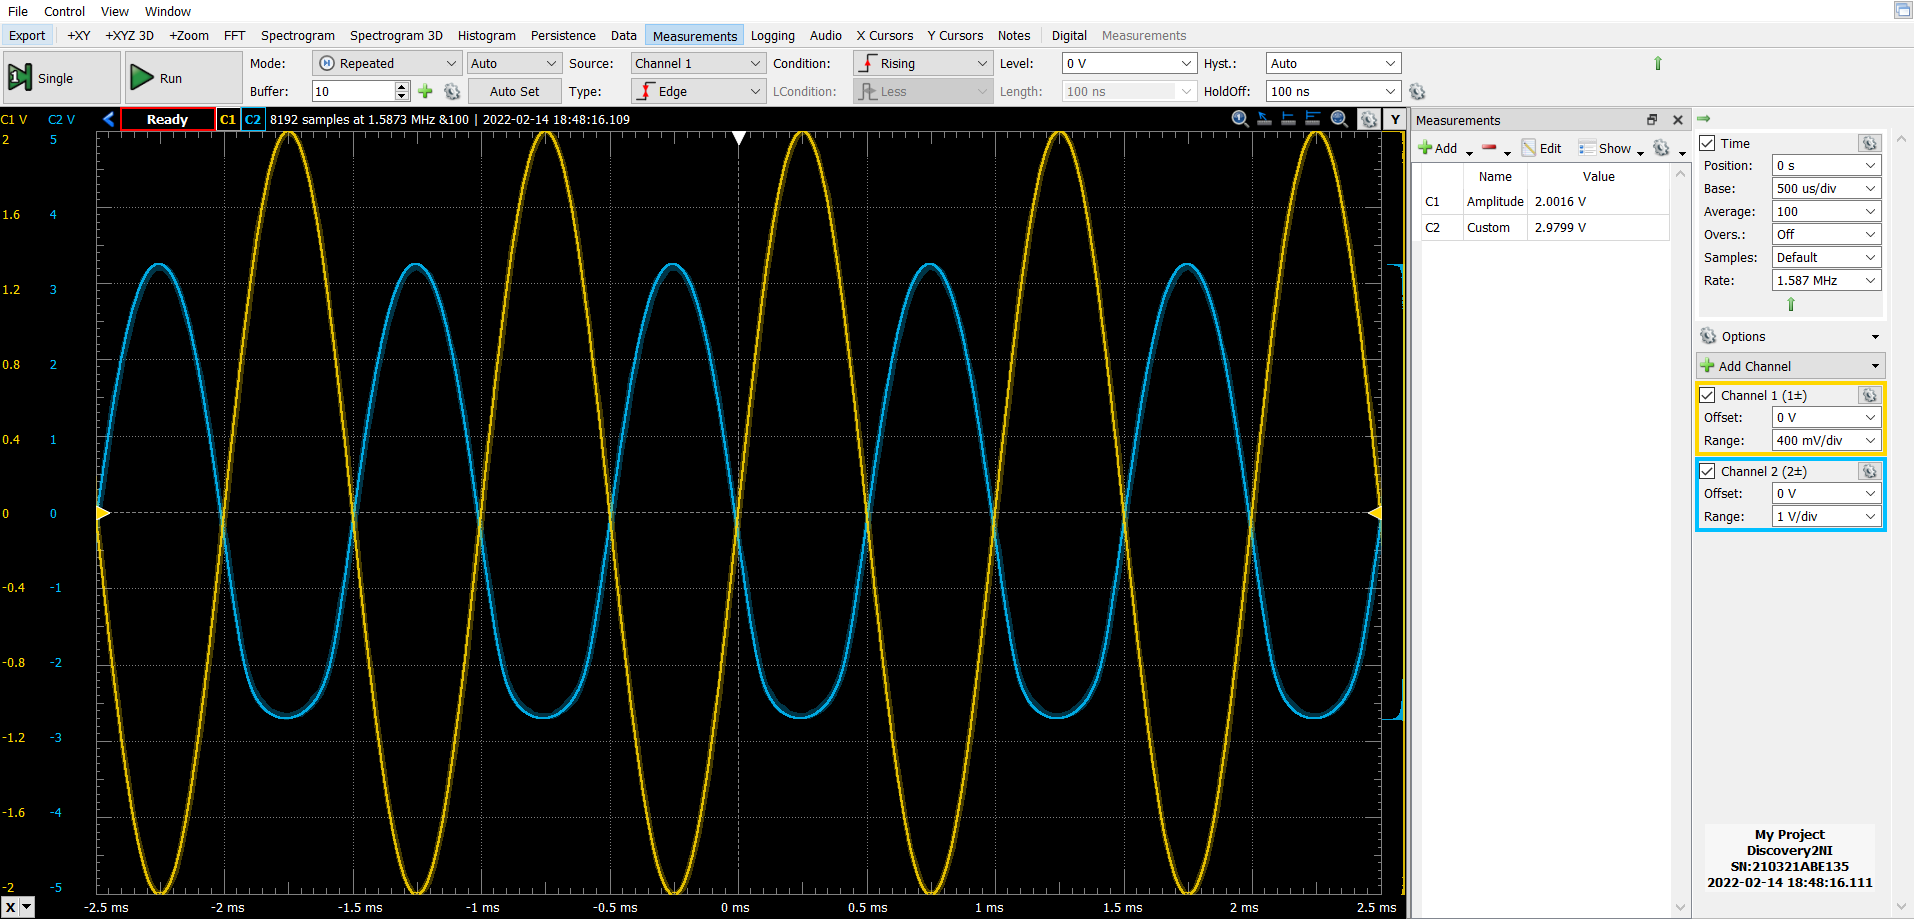
\includegraphics[width=\textwidth]{amp.2000}
    \caption{Acquisizione all'oscilloscopio di $v\ped{in} (t)$ (CH1) e
    $v\ped{out} (t)$ (CH2) in funzione del tempo con ampiezza
    $v\ped{in} = 2 \; \si{\V}$. In cui la distorsione della parte inferiore
    dell'onda per effetto di clipping è molto più pronunciata}
\end{figure}
\begin{figure}[htbp]
    \centering
	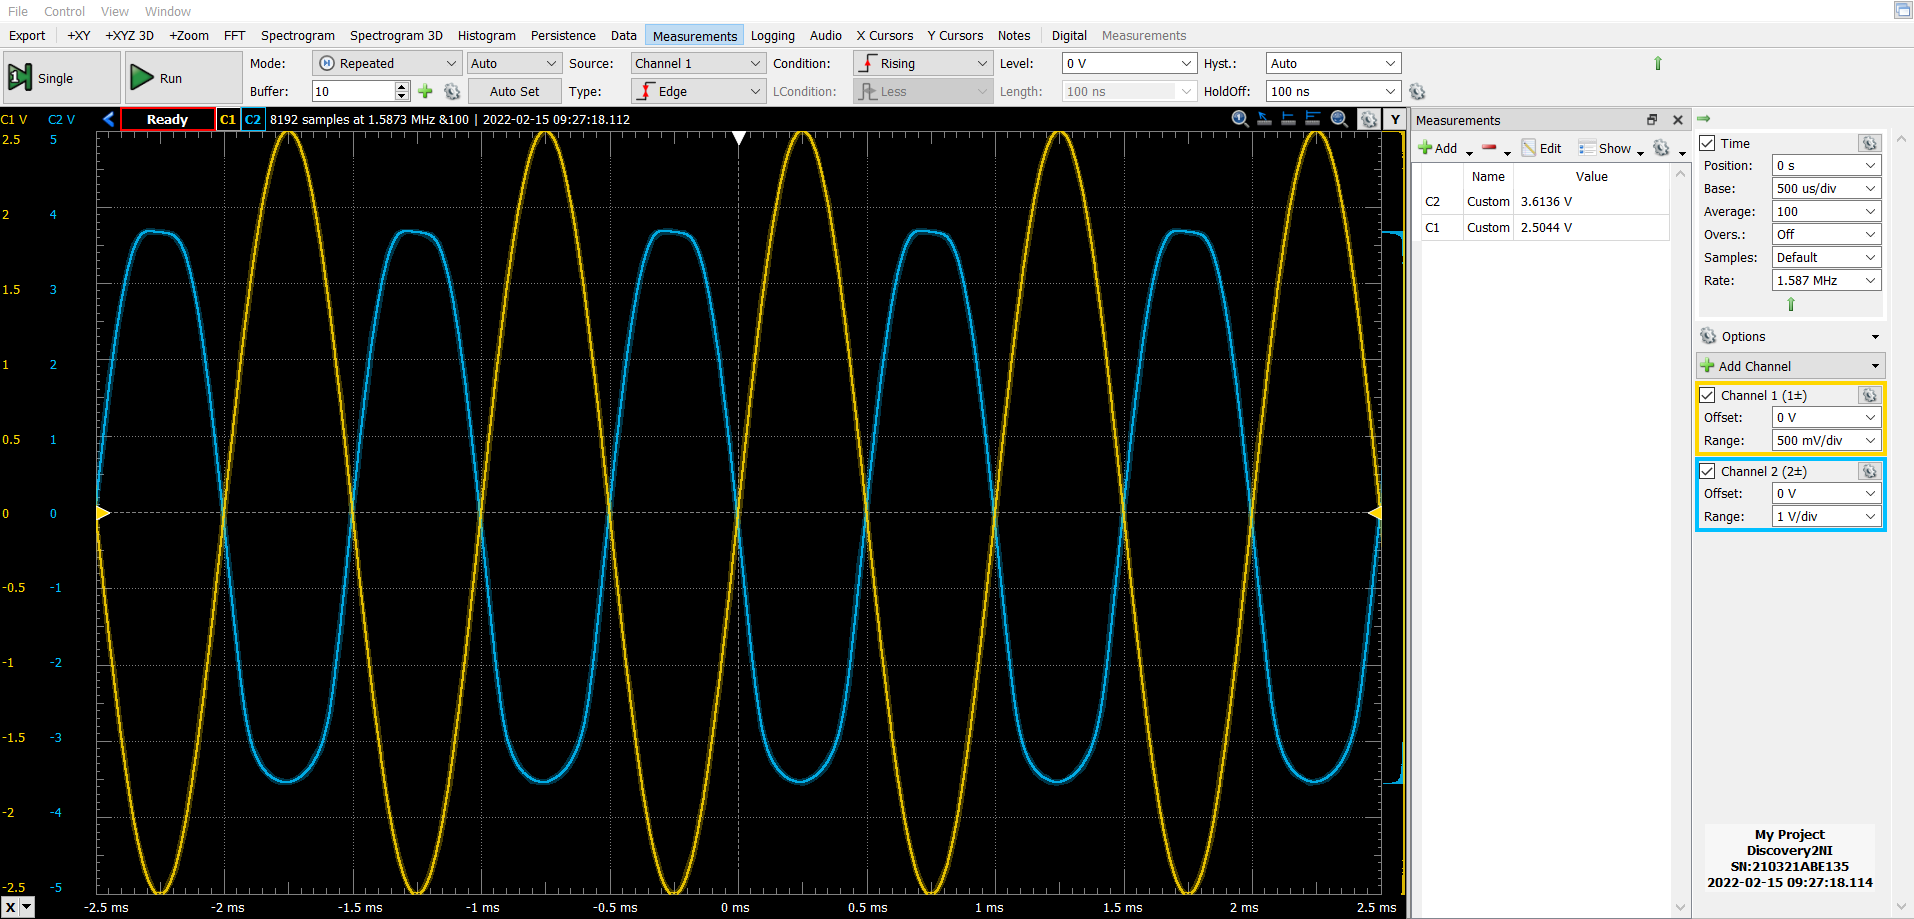
\includegraphics[width=\textwidth]{amp.2500}
    \caption{Acquisizione all'oscilloscopio di $v\ped{in} (t)$ (CH1) e
    $v\ped{out} (t)$ (CH2) in funzione del tempo con ampiezza
    $v\ped{in}=2.5 \; \si{\V}$; si inizia a intravedere un taglio nella parte
    superiore dell'onda, mentre la parte inferiore risulta ancora distorta}
\end{figure}
\begin{figure}[htbp]
    \centering
	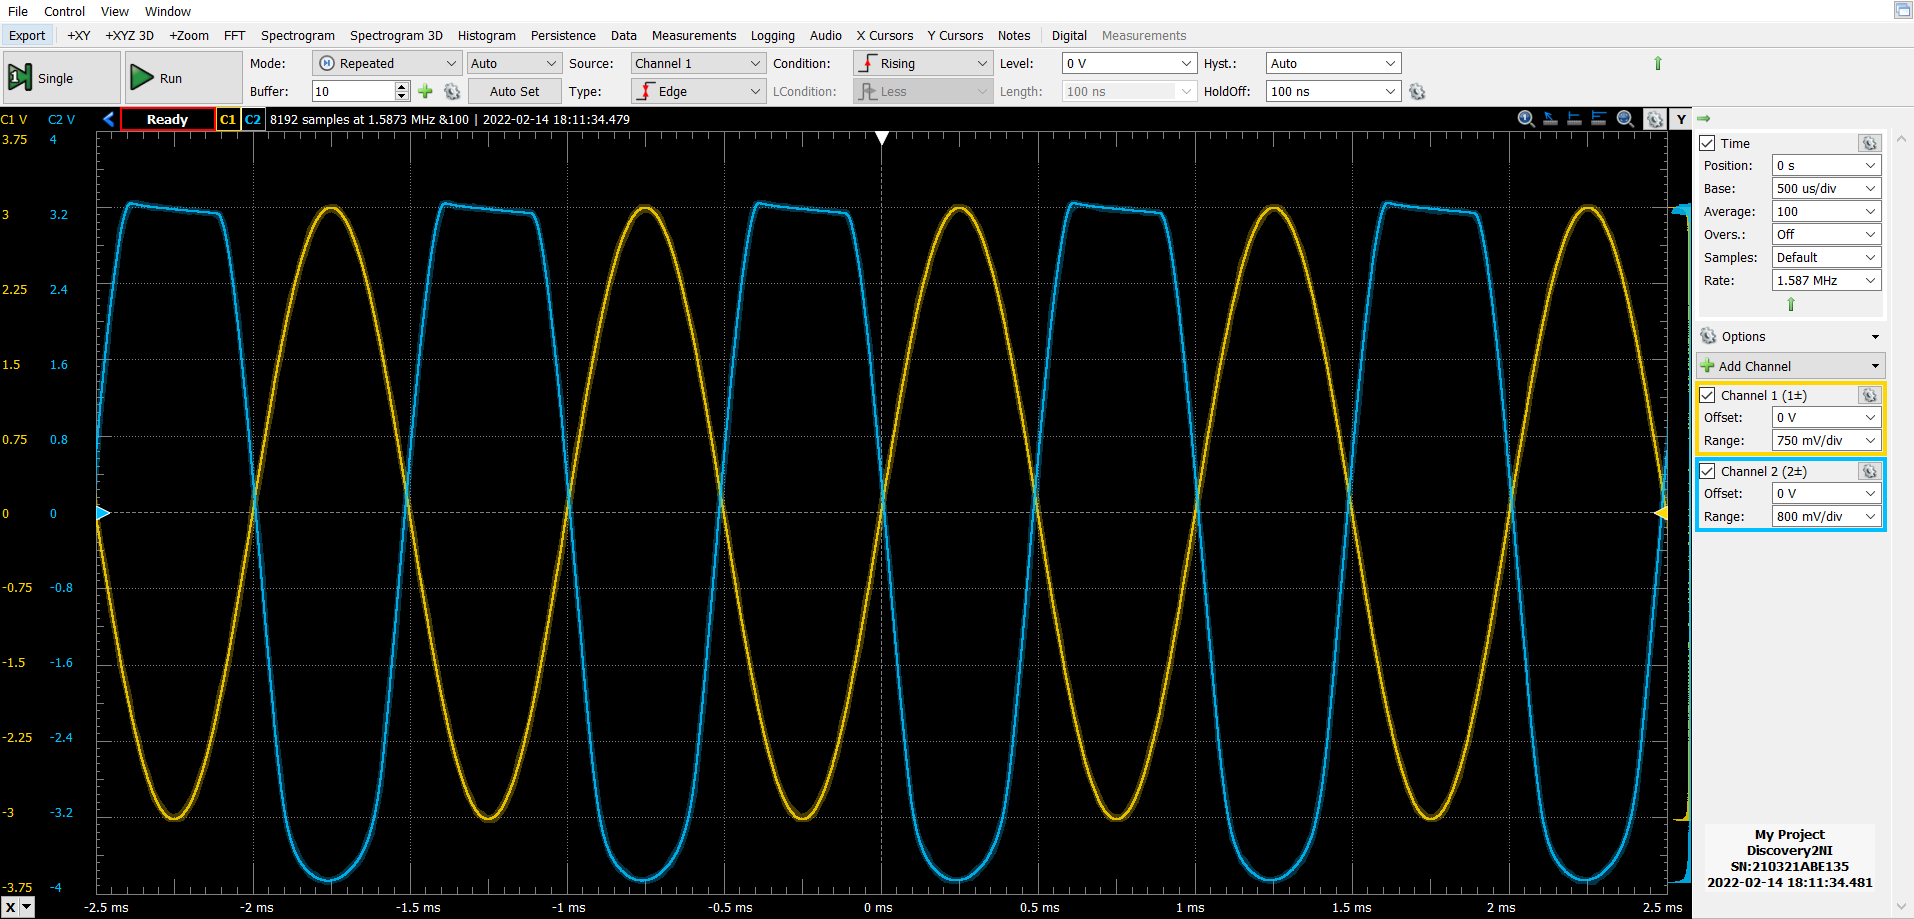
\includegraphics[width=\textwidth]{amp.3000}
    \caption{Acquisizione all'oscilloscopio di $v\ped{in} (t)$ (CH1) e
    $v\ped{out} (t)$ (CH2) in funzione del tempo con ampiezza
    $v\ped{in} = 3 \; \si{\V}$; il taglio della parte alta dell'onda risulta
    ora più evidente}
\end{figure}

Dalle nostre misure notiamo una deviazione significativa dal regime di
amplificazione lineare (definibile arbitrariamente come una deviazione di più
di 3 barre d'errore rispetto al valore di guadagno atteso) quando l'ampiezza
del segnale in ingresso risulta compatibile con la tensione $V_{GS}$. Questo
risulta ragionevole, dal momento che -quando la piccola tensione di disturbo
$v\ped{in}$ è abbastanza grande da condurre il JFET fuori dal regime di
saturazione- cessa di essere valida relazione che lega l'intensità della
corrente erogata dal generatore variabile (che scorre dal drain verso il
source) alla tensione tra gate e source $i_{ds} = -g_m v_{gs}$.

A maggior ragione non possono continuare ad essere valide le espressioni
attese per il guadagno dell'amplificatore che discendono da questa
\[
\begin{dcases}
v\ped{in} = v_{gs} + R_S i_{ds} \\
%
v\ped{out} = - R_D i_{ds} = - R_D g_m v_{gs} \\
\end{dcases}
\: \implies A_v = \frac{v\ped{out}}{v\ped{in}} =
- \frac{g_m R_D}{1 + g_m R_S}
\]
%=======================
\section{Risposta in frequenza}
\subsection{Network Analyzer}
Si è inviato come segnale in ingresso all'amplificatore a emettitore comune una
sinusoide di frequenza compresa tra $\SI{5}{\Hz}$ e $\SI{10}{M\Hz}$ di
ampiezza costante pari a $v\ped{in} = 200 \; \si{m\V}$ e si è registrata la
risposta in frequenza del sistema monitorandone l'uscita in $v\ped{out}$ con
lo strumento Network dell'AD2
\begin{figure}[htbp]
    \centering
	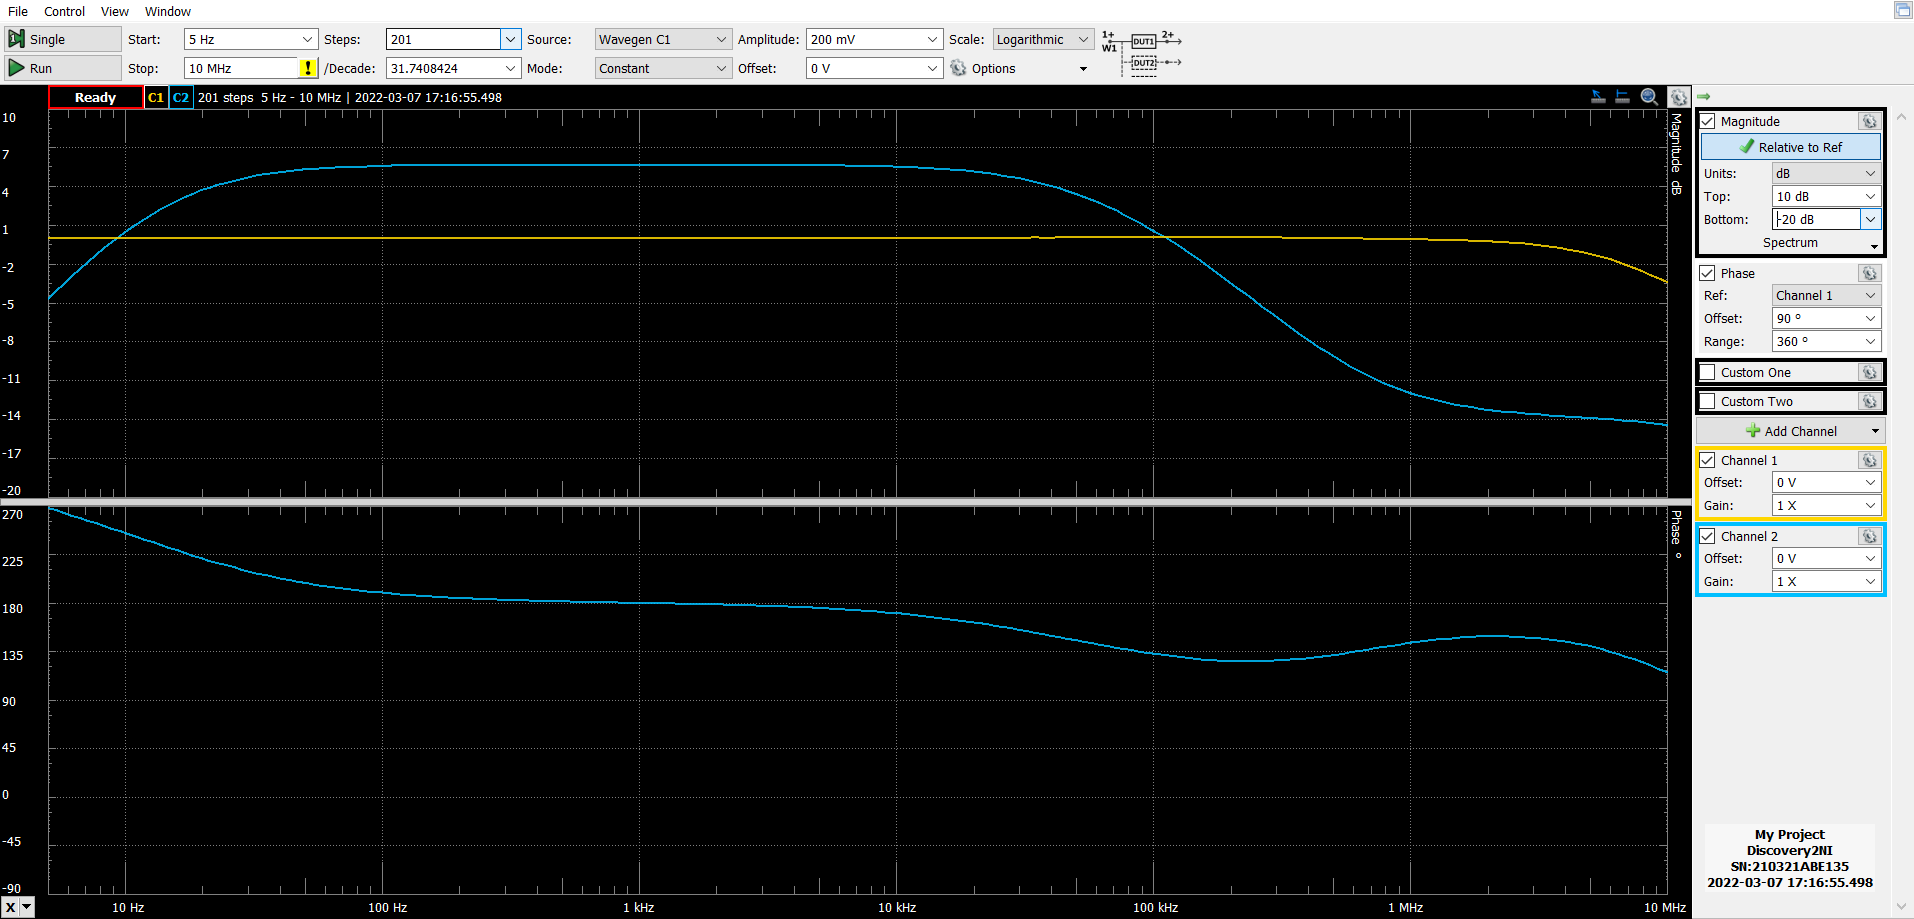
\includegraphics[width=\textwidth]{net}
    \caption{Plot di Bode ottenuto dallo scan con Network tra $5 \; \si{\Hz}$ e
$\SI{10}{M\Hz}$ con un segnale sinusoidale in ingresso di ampiezza costante
$v\ped{in} = \SI{200}{m\V}$. \label{fig: bodeplot}}
\end{figure}

Si è quindi misurato il guadagno di centro banda con i cursori, che risulta
essere pari a
\[
A_v = 6.31 \pm 0.07 \; \si{dB} = 2.07 \pm 0.02
\]
quindi compatibile con quanto misurato al punto precedente.

\subsection{Misura delle frequenze di taglio}\label{sbs: fT}
Partendo dalla misura del guadagno a centro banda, possiamo
ottenere una stima del valore delle frequenze di taglio a bassa $f_L$ e ad
alta frequenza $f_H$ dai punti in cui il guadagno diminuisce di un fattore
$1/\sqrt{2}$, cioè di circa $-3.01 \; \si{dB}$ rispetto ad $A_v$.
\begin{align*}
F_{H} &= 3.54 \pm 0.02 \; \si{M\Hz} \\
F_{L} &= 16.0 \pm 0.1 \; \si{\Hz}
\end{align*}

Trascurando le capacità delle giunzioni nel transistor ci aspettiamo che la
frequenza di taglio ``bassa'' corrisponda a quella di un filtro passa-alto
costituito dalla serie $C\ped{in} + R_G$:
\begin{equation}
\frac{1}{2\pi R_G C\ped{in}} = 1.64 \pm 0.07 \; \si{\Hz}
\end{equation}

La misura della frequenza di passa alto non risulta compatibile con il suo
valore atteso, anzi, i due risultati differiscono per un fattore di scala di
circa 10.

Nella configurazione ad emettitore comune con guadagno superiore all'unità,
l'impedenza in uscita dell'amplificatore risulta sempre più grande al
crescere del guadagno (in valore assoluto). Per cui, dal Teorema di Miller ci
aspettiamo che anche le piccole capacità parassite (dell'ordine del pF) tra
gate e canale portino ad una sensibile diminuzione del guadagno come quella
osservata all'aumentare della frequenza, per $f \gg f_{H}$.

Possiamo provare a dare una stima dell'ordine di grandezza della capacità
parassita $C_p$ corrispondente alla frequenza di taglio ``alta'' trovata;
sapendo che la resistenza in uscita è data da $R_D$ ci aspettiamo
\[
C_p = \frac{1}{2\pi R_C f_H} = 45.0 \pm 0.3 \; \si{p\F}
\]
che seppur non dello stesso ordine di grandezza dei valori di capacità
tipiche riportate nel datasheet del 2N3819, come prima non se ne discosta per
molto più di un fattore 10.

%=======================
\section{Aumento del guadagno con passa-alto all'emettitore}
\subsection{Modifica del ramo di emettitore}
Inserendo il condensatore elettrolitico $C_S$ in parallelo con $R_S$ viene a
modificarsi l'impedenza del ramo di emettitore che diminuisce, aumentando di
conseguenza il guadagno come in:
\begin{equation}\label{eq: AvCS}
A_v = -\frac{g_m R_D}{1 + g_m |Z_S|}
\end{equation}
dove $Z_S$ è l'impedenza data dal parallelo di $R_S$ e $C_S$:
\begin{equation}
Z_S(\omega) = \frac{R_S}{j\omega C_S R_S +1}
\end{equation}

Calcolandone il modulo si ottiene un valore di resistenza parallelo
$\abs{Z_S} = 1.68 \pm 0.09 \ohm$ per una frequenza di 1 kHz.
Dunque possiamo ricalcolare il guadagno atteso dalla \cref{eq: AvCS}, che
per la stessa frequenza ora risulta pari a
\[
A_v = 3.88 \pm 0.06
\]

\subsection{Misura del guadagno con $C_S$}
A questo punto siamo passati a prendere delle misure per il guadagno per un
piccolo segnale sinusoidale a frequenza $f = \SI{1}{k\Hz}$ con un'ampiezza in
ingresso $v\ped{in} = 100 \; \si{m\V}$, da cui otteniamo
\[
A_v = \frac{v\ped{out}}{v\ped{in}} = 3.89 \pm 0.05
\].
Risultato compatibile entro una barra di errore con l'aspettativa\footnote{
Per effettuare al meglio questa misura è stato necessario agire più volte sul
circuito, smontandolo e rimontandolo in seguito, e spostando i componenti
(lasciando invariata la schematica), perché lo stesso era estremamente
instabile e il fattore di amplificazione cambiava notevolmente anche al più
piccolo urto sul tavolo, rendendo da quel momento in poi impossibile
effettuare la misura.}.
\begin{figure}[htbp]
    \centering
	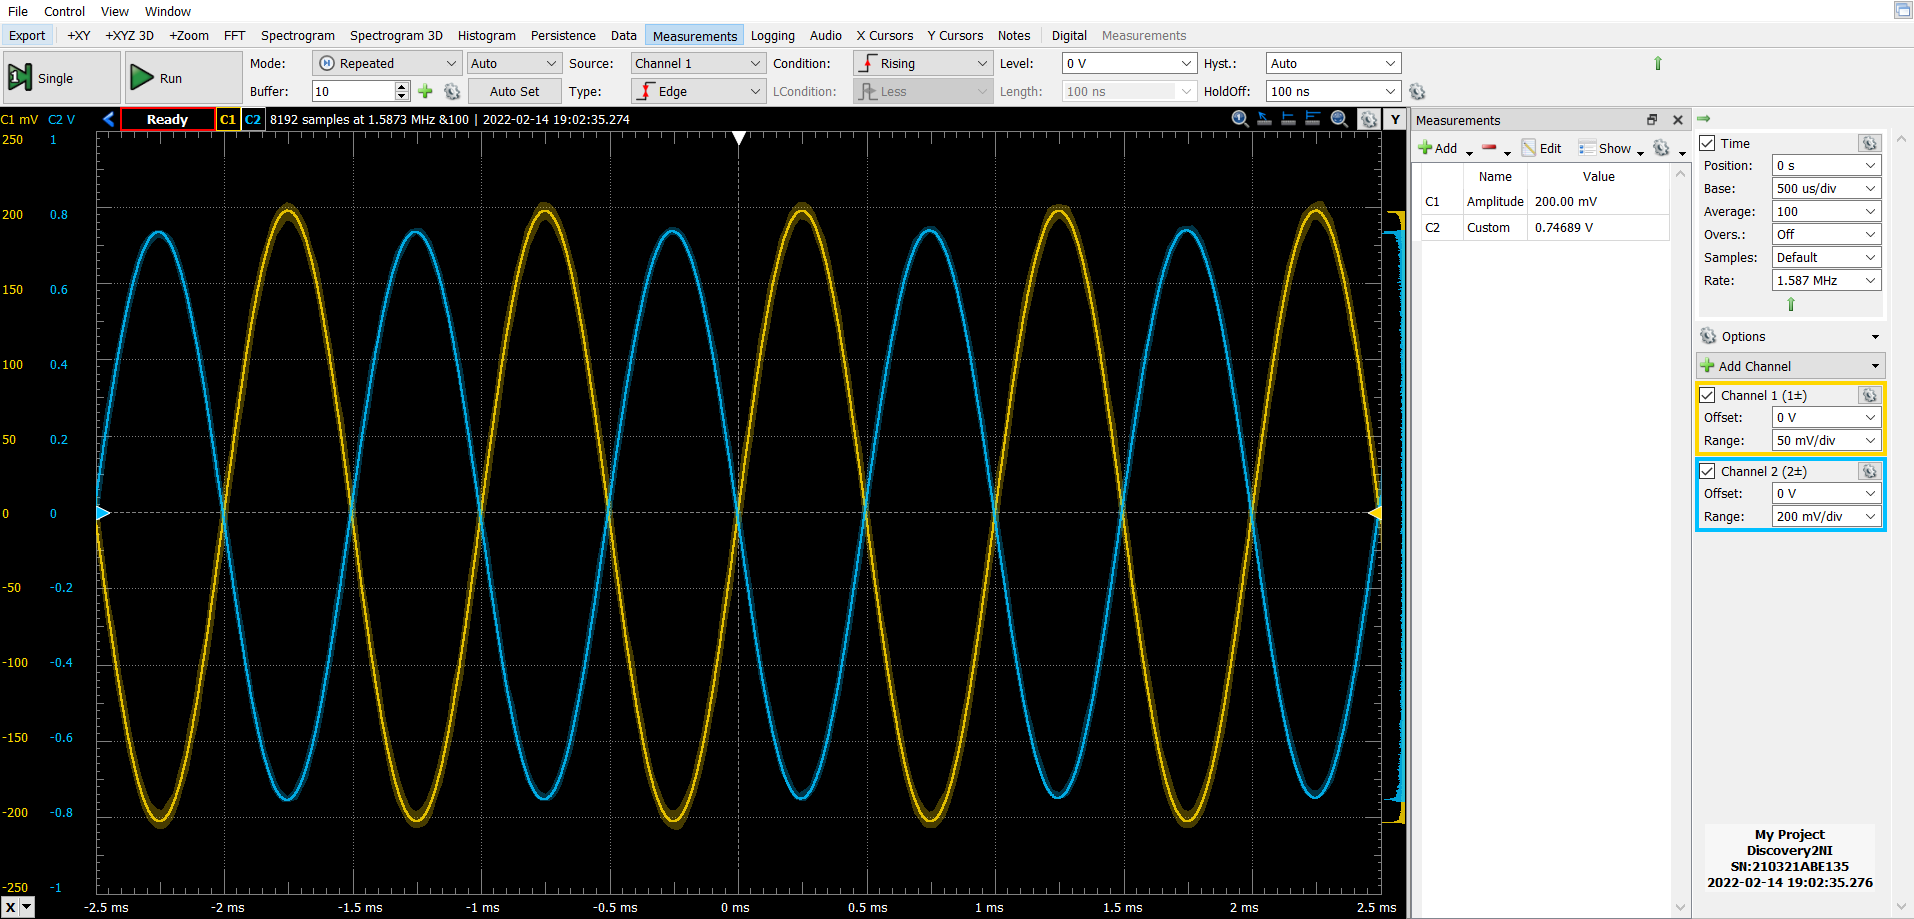
\includegraphics[width=\textwidth]{amp.200.cap}
    \caption{Acquisizione presa dall'oscilloscopio dell'andamento nel tempo
    dei segnali $v\ped{in} (t)$ (CH1) e $v\ped{out} (t)$ (CH2) con ampiezza
    $v\ped{in} = 200 \; \si{m\V}$ con condensatore elettrolitico $C_S$ in
    parallelo a $R_S$}
\end{figure}

%=======================
\section{Impedenza in ingresso}
\subsection{Stima dell'impedenza in ingresso}
Si è infine provato a misurare l'impedenza in ingresso al circuito inserendo
tra il generatore e l'ingresso dell'amplificatore una resistenza $R_S$ dello
stesso ordine di grandezza dell'impedenza in ingresso attesa per il circuito
$Z\ped{in} \approx R_G \sim \SI{1}{M\ohm}$.

\subsection{Impedance Analyzer}
Utilizzando lo strumento Impedance Analyzer dell'AD2 in configurazione
``W1-C1-R-C2-DUT-GND'' si è potuto visualizzare l'andamento in frequenza
dell'impedenza $Z\ped{in}$ e la reattanza in parallelo $X_P$ in un intervallo
compreso tra 1 e $10 \; \si{k\Hz}$.
\begin{figure}[htbp]
    \centering
	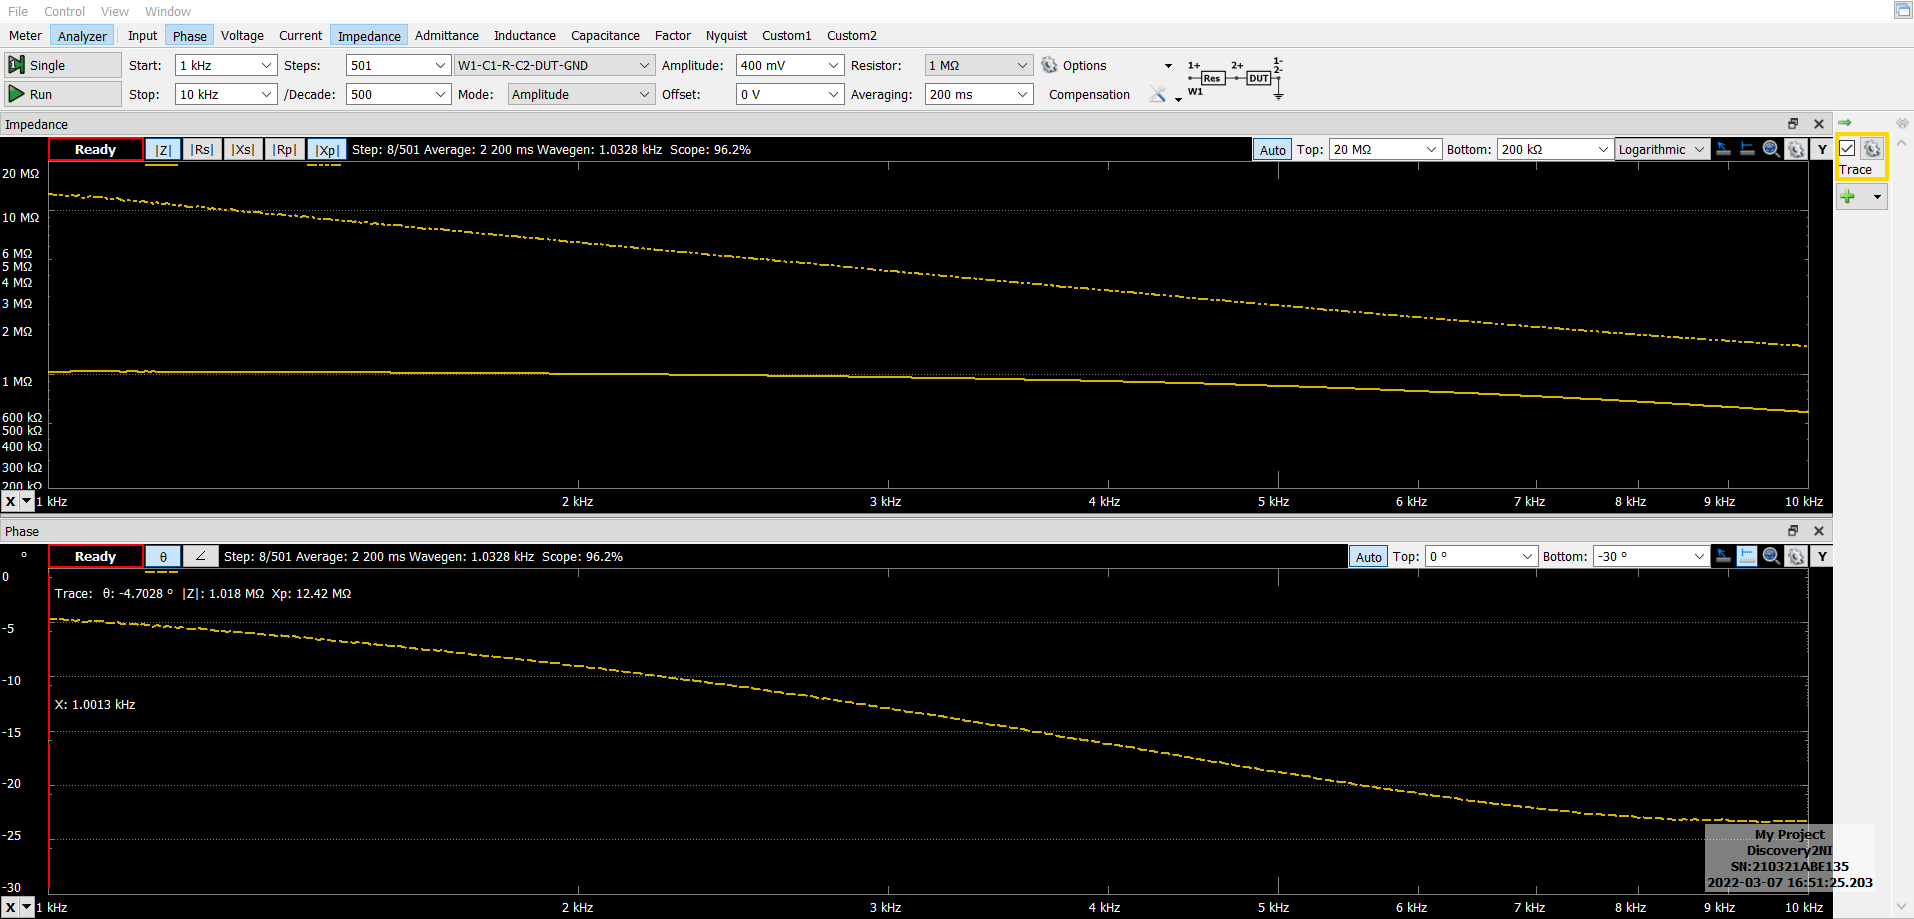
\includegraphics[width=\textwidth]{amp}
    \caption{Grafici di impedenza in ingresso e reattanza parallelo in
    funzione della frequenza per $R_S = 1 \si{M\ohm}$}
\end{figure}

\subsection{Confronto le caratteristiche del JFET reale}
Ipotizziamo che l'andamento simile ad un passa-basso trovato per l'impedenza
dipenda ancora una volta dalla presenza di capacità parassite tra le zone di
svuotamento e il canale in parallelo di cui si è provato a dare una stima in
\cref{sbs: fT}.

%=======================
\section*{Conclusioni e commenti finali}
Si è riusciti a costruire e caratterizzare un amplificatore di tensione
invertente con un JFET in configurazione a emettitore comune. In particolare
si è riusciti ad apprezzare il differente comportamento (anche non lineare)
del circuito in vari regimi, dare una stima di guadagno, impedenza in
ingresso e frequenze caratteristiche della sua risposta in frequenza.

%=======================
\section*{Dichiarazione}
I firmatari di questa relazione dichiarano che il contenuto della relazione \`e
originale, con misure effettuate dai membri del gruppo, e che tutti i firmatari
hanno contribuito alla elaborazione della relazione stessa.

\end{document}
